% =====================================================================
\section{Thảo luận}
% =====================================================================
 
\subsection{So sánh bốn phương pháp}
 
\paragraph{Độ chính xác và thiên kiến mô hình.} Thứ tự accuracy phản ánh mức độ linh hoạt của biên quyết định. Naive Bayes và Logistic Regression đều có biên \emph{tuyến tính} trong không gian pixel (điểm số NB $s_c=\log\pi_c+\mathbf{x}^\top\log\boldsymbol\theta_c$ cũng tuyến tính theo $\mathbf{x}$), nhưng NB ước lượng tham số theo giả định độc lập pixel và không tối ưu trực tiếp cho phân lớp, còn LR tối ưu cross-entropy một cách phân biệt. Cùng một họ biên tuyến tính, LR giảm lỗi test từ 1\,636 xuống 787, tức hơn một nửa. Cả hai có khoảng cách train--test gần 0: đây là \emph{underfit}, mô hình quá đơn giản chứ không phải học thuộc. MLP và Random Forest có biên phi tuyến, đạt 96--98\% nhưng đổi lại khoảng cách train--test lớn hơn (1.9 và 3.3 điểm).
 
\paragraph{MLP so với Random Forest.} Hai mô hình phi tuyến đều gần như thuộc lòng tập train, nhưng MLP tổng quát hoá tốt hơn: lỗi test 191 so với 355. Mỗi nút của cây chỉ hỏi \emph{một} pixel so với một ngưỡng, nên biên quyết định gồm các mặt cắt song song trục; một nét bút dịch đi 1--2 pixel làm thay đổi hàng loạt câu trả lời. Các nơ-ron ẩn của MLP là tổ hợp tuyến tính của mọi pixel, học được các ``mẫu nét'' bền hơn với biến dạng nhỏ. Recall của MLP cũng đồng đều nhất giữa các lớp (0.974--0.995), trong khi Random Forest có các lớp 7, 8, 9 thấp hơn hẳn lớp 0, 1.
 
\paragraph{Chi phí và khả năng diễn giải.}
\begin{table}[H]
\centering\small
\caption{So sánh thực tiễn bốn bộ phân lớp (cấu hình cuối).}\label{tab:practical}
\begin{tabular}{@{}lcccl@{}}
\toprule
Mô hình & Test acc. & Dự đoán (ms/ảnh) & Kích thước file & Diễn giải \\
\midrule
Multinomial NB      & 0.836 & 0.007 & 0.1\,MB  & bản đồ $\theta_c$, hiệu $\log\theta_7-\log\theta_1$ \\
Logistic Regression & 0.921 & 0.002 & 0.1\,MB  & trọng số mỗi lớp vẽ thành ảnh \\
MLP                 & 0.981 & 0.002 & 1.9\,MB  & khó, chỉ gián tiếp \\
Random Forest       & 0.965 & 0.206 & 35.1\,MB & feature importance từng pixel \\
\bottomrule
\end{tabular}
\end{table}
Naive Bayes huấn luyện tức thì (một lượt cộng dồn) và không có siêu tham số nhạy cảm, phù hợp làm đường cơ sở. Random Forest không cần chuẩn hoá dữ liệu, không cần learning rate, có OOB score miễn phí, nhưng là mô hình nặng nhất: file 35\,MB (lưu hàng chục nghìn nút) và dự đoán chậm hơn MLP khoảng 100 lần do duyệt cây bằng vòng lặp Python. MLP cho accuracy cao nhất với chi phí dự đoán ngang mô hình tuyến tính, đổi lại cần chọn learning rate, kiến trúc và dừng sớm, và khó diễn giải nhất.
 
\subsection{Phân tích lỗi}
 
\paragraph{Các cặp nhầm có nguyên nhân hình học.} Bảng~\ref{tab:pairs} cho thấy các cặp hay nhầm giống nhau giữa các mô hình, chỉ khác về độ lớn. $4\leftrightarrow9$ là cặp khó nhất ở mọi mô hình: chữ 4 viết ``đóng'' phần trên gần như trùng chữ 9, chỉ khác nét nối nhỏ ở đỉnh. $3\leftrightarrow5$ và $7\leftrightarrow9$ chia sẻ phần lớn nét (đường cong dưới của 3 và 5; nét chéo của 7 và thân 9). Điều này khớp với EDA: ảnh trung bình của các cặp này giống nhau nhất.
 
\paragraph{Vì sao Naive Bayes lỗi theo kiểu ``hút về một lớp''.} Điểm NB là tổng mực có trọng số $\log\theta_{cj}$, nên lớp có ``bản đồ mực'' rộng và phủ nhiều vùng (8 phủ gần hết vùng tâm, 9 phủ phần trên và thân) nhận điểm cao cho rất nhiều ảnh lạ, giải thích cột 8 và cột 9 nhận nhiều lỗi. Chữ 5 bị đoán thành 3 (107 lần) vì phần dưới hai chữ gần trùng, còn phần trên khác biệt chỉ chiếm ít pixel. Giả định độc lập pixel không cho NB nhận ra rằng một nét nối liền (đặc trưng của 4 mở so với 9 đóng) quan trọng hơn tổng lượng mực.
 
\paragraph{Random Forest và lỗi $7\to2$.} Random Forest có lỗi $7\to2$ (26 ảnh) nhiều hơn cả Logistic Regression (21). Chữ 7 có gạch ngang giữa hoặc nét dưới cong sang phải có phân bố pixel giống chữ 2 ở phần dưới ảnh; vì mỗi nút chỉ xét một pixel, các cây dễ ``rẽ'' theo vài pixel ở đáy ảnh. Đây là biểu hiện của tính nhạy với vị trí nét đã nêu ở trên.
 
\begin{figure}[H]
\centering
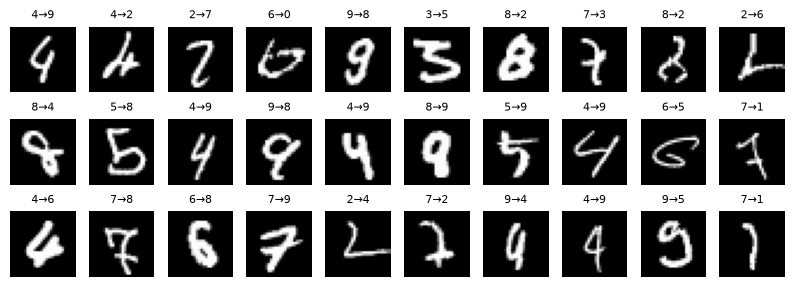
\includegraphics[width=0.9\textwidth]{figures/errors_test.png}
\caption{30 ảnh test đầu tiên bị MLP (mô hình tốt nhất) đoán sai, ghi ``nhãn thật $\to$ dự đoán''.}\label{fig:errors}
\end{figure}
 
\paragraph{Lỗi còn lại của MLP phần lớn là ảnh thật sự mơ hồ.} Trong Hình~\ref{fig:errors}, nhiều ảnh khó với cả người đọc: các chữ 4 có đỉnh khép kín bị đọc là 9 (xuất hiện 5 lần trong 30 ảnh), chữ 2 viết như chữ L (bị đọc thành 6 hoặc 4), chữ 6 viết nghiêng như số 0 hoặc 5, chữ 7 có gạch ngang đọc thành 2 hoặc 3. Một số ảnh có thể bị gán nhãn sai từ gốc. Với 191 lỗi trên 10\,000 ảnh, phần cải thiện còn lại khó đạt được bằng mô hình chỉ nhìn pixel độc lập vị trí như MLP.
 
\subsection{Hạn chế}
 
\begin{itemize}
\item \textbf{Tìm kiếm siêu tham số hạn chế.} Mỗi mô hình chỉ quét một siêu tham số chính. Random Forest cố định \code{max\_depth}$=15$, \code{min\_samples\_leaf}$=1$ và \code{max\_features}$=\sqrt D$ vì chi phí huấn luyện; chưa thử \code{"log2"}, cây sâu hơn hay lá lớn hơn, nên khoảng cách train--test 3.3 điểm có thể còn thu hẹp được. MLP chưa quét learning rate và $\lambda$ (cấu hình cuối dùng $\lambda=0$). Đường theo số cây chỉ lấy từ một rừng, một hạt giống.
\item \textbf{Một lần chia dữ liệu, một hạt giống cho cấu hình cuối.} Accuracy test báo cáo từ một lần huấn luyện; không có khoảng tin cậy. Với 10\,000 ảnh test, sai số chuẩn của accuracy khoảng $\sqrt{p(1-p)/10^4}\approx0.13$--0.37 điểm phần trăm, nên chênh lệch giữa các mô hình trong báo cáo đều có ý nghĩa, nhưng chênh lệch nhỏ khi đối chiếu với thư viện (Bảng~\ref{tab:sklearn}) nằm trong biên độ ngẫu nhiên. Mô hình cuối chỉ huấn luyện trên 54\,000 ảnh, chưa gộp lại validation.
\item \textbf{Hiệu năng cài đặt Random Forest.} Dự đoán bằng vòng lặp Python từng ảnh làm Random Forest chậm nhất (0.2\,ms/ảnh) và huấn luyện tuần tự từng cây (khoảng 9\,s/cây, $\approx$7.5 phút cho 50 cây). Có thể vector hoá việc duyệt cây bằng cách lưu cây dạng mảng và xử lý theo lô, hoặc huấn luyện song song các cây vì chúng độc lập.
\item \textbf{Biểu diễn đầu vào thô.} Cả bốn mô hình nhìn ảnh như vector 784 pixel độc lập vị trí. Thí nghiệm độ bền trong notebook cho thấy khi dịch ảnh 3 pixel theo đường chéo, accuracy test giảm còn 0.11--0.20 với cả bốn mô hình không dùng tăng cường dữ liệu; tăng cường dữ liệu nâng MLP lên 0.78 nhưng Random Forest chỉ lên 0.37. Mạng tích chập (CNN) với tính bất biến tịnh tiến sẵn có mới giải quyết triệt để vấn đề này.
\item \textbf{Lệch miền.} Trên tập 2\,980 chữ số do 30 người Việt viết (đánh giá trên phần người viết giữ lại, trung bình 3 lần chia), accuracy khi chỉ huấn luyện bằng MNIST giảm mạnh: MLP 0.894, Random Forest 0.688, Logistic Regression 0.690, NB 0.575. Kết quả trên MNIST vì vậy đánh giá quá cao khả năng dùng thực tế; Random Forest giảm nhiều nhất (từ 0.962 xuống 0.688), nhất quán với nhận xét về độ nhạy theo vị trí pixel.
\item \textbf{Giả định của Naive Bayes.} Coi cường độ pixel thực là ``số đếm'' và giả định pixel độc lập đều không đúng với ảnh chữ viết, nơi các pixel lân cận tương quan mạnh. Đây là giới hạn của mô hình, không phải của cài đặt (đã khớp tuyệt đối với scikit-learn).
\end{itemize}